\chapter{DemoA} \label{ch:DemoA}


\section{Introduction}
Welcome to the demo of Verefoo for VPNs. What you will see written here will be a simple stand-alone demo in which the features and capabilities of Verefoo are highlighted.
Before we begin we need to define a network topology that Verefoo will need to relate to, more precisely you will also need to define the respective IP addresses and links between the different nodes.  During the course of the demo, a virtual environment developed with Docker Containers will be instantiated that will reproduce the topology presented in this document.

\begin{figure}[h]  % 'h' significa che la figura viene posizionata qui
    \centering
    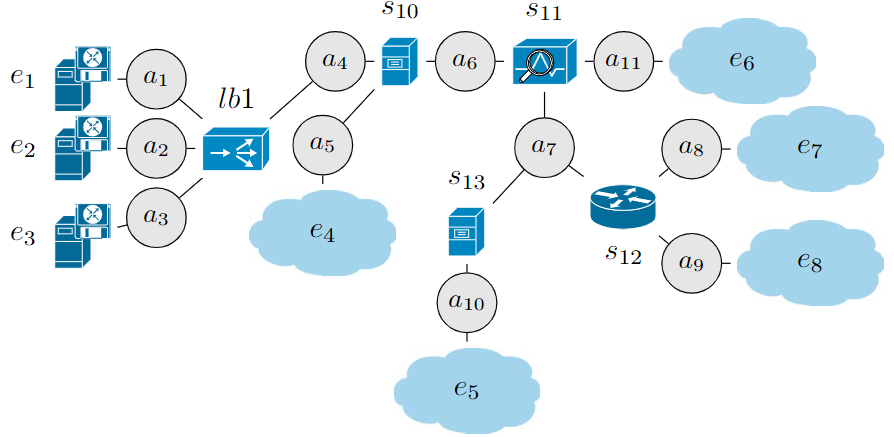
\includegraphics[width=1\textwidth]{VPN_AG.PNG} 
    \caption{Service Graph}
    \label{fig:ServiceGraph}
\end{figure}
As can be seen, the proposed topology has 3 webservers on the left whose traffic is handled by a load balancer and 5 endpoints that are represented by web clients. Within the network there are nodes that will act as monitors, such as node s11, and others that will instead perform the simple forwarder function with their respective static routes. Finally, there are several currently empty nodes that we will call allocation places. Within these nodes, the framework will be able to place network security functions to make sure that the security requirements are working properly within the network. A table is provided below with the definition of each node, its IP address that will be used in the virtual environment, and its functionality within the topology.

\begin{table}[h]
    \centering
    \begin{tabular}{ccc}
        \hline
         Name & IP & Functionality \\
        \hline
        e1 & 130.10.0.1 & Web servers behind load balancer b1 \\
        e2 & 130.10.0.2 & * \\
        e3 & 130.10.0.* & * \\
        e4 & 40.40.41.* & Web Client \\ 
        e5 & 40.40.41.* & Web Client \\
        e6 & 88.80.84.* & Web Client \\
        e7 & 192.168.1.* & Web Client \\
        e8 & 192.168.2.* & Web Client \\
        lb1 & 130.10.0.4 & Load Balancer \\
        s10 & 33.33.33.2 & Web Cache \\
        s11 & 33.33.33.3 & Forwarder \\
        s12 & 220.124.30.1 & Forwarder \\
        s13 & 33.33.33.4 & Forwarder \\
        a7 & 1.0.0.7 & Forwarder \\
        \hline
    \end{tabular}
    \caption{Node definitions and functionalities}
    \label{tab:tabella}
\end{table}


The second and final input that must be provided to the framework is the set of security requirements that the network must have. With this demo, the goal was to have an output topology that contained a large number of VPN Gateways (6), in order to be able to show an example that would come as close as possible to a hypothetical real case of a small-to-medium sized company. In order to be able to achieve a similar topology, the following rules were defined:
\\
\\

\begin{table}[h]
    \centering
    \small
    \begin{tabular}{ccccccccc}
        \hline
         Policy & IPSrc & IPDst & pSrc & pDst & tProto & Confidentiality & Intregrity & Untrusted nodes\\
        \hline
        Protection & 40.40.41.1 & 130.10.0.1 & * & 22 & ANY & AES-256-CBC & SHA2-256 & 33.33.33.2 \\
        Protection & 88.80.84.1 & 130.10.0.* & * & 80 & ANY & AES-256-CBC & SHA2-256 & 33.33.33.2/33.33.33.3 \\
        Protection & 192.168.1.1 & 130.10.0.1 & * & * & ANY & AES-256-CBC & SHA2-256 & 33.33.33.2/33.33.33.3 \\
        Protection & 40.40.42.1 & 192.168.2.1 & * & * & ANY & AES-256-CBC & SHA2-256 & 33.33.33.4/220.124.30.1 \\
        \hline
    \end{tabular}
    \caption{Security Requirements Definition}
    \label{tab:tabella}
\end{table}
\begin{itemize}
    \item \textbf{First Rule}: Web Client e4 must be able to communicate securely with Web Server e1. Traffic originating from e4 can use any port for the transport protocol but the e5 Server must receive data only from port 22. Both UDP and TCP protocols can be used for communications. Finally, node s10 is specified as a non-secure node and through which traffic must pass encrypted.
    \item \textbf{Second Rule}: Web Client e8 must be able to communicate securely with all Web Servers (e1,e2,e3). Traffic originating from e8 can use any port for the transport protocol but the servers must receive data only from port 80. It is possible to use either UDP or TCP protocol for communication. In this case the nodes that are considered non-secure are s10 and s11.
    \item \textbf{Third Rule}: Web Client e7 must be able to communicate securely with Web Server e1. There are no limitations on ports for incoming and outgoing traffic, and any fourth-level protocol can be used. The unsecured nodes, as with the second rule, are s10 and s11. 
    \item \textbf{Fourth Rule}:The Web Client e5 must be able to communicate securely with the Web Client e8. As with the third rule, there are no limitations on the ports and transport protocol to be used. The nodes considered insecure for this rule are s12 and s13.
\end{itemize}

\section{Output}
By providing the previously defined inputs, the framework will look for a solution that not only satisfies all the rules, but also employs the least amount of resources necessary to guarantee these properties. Verefoo will then solve a problem defined as MaxSMT (Maximum Satisfiability Modulo Theories). 
In the specific case of this demo, the result produced in output will be as follows:

\begin{figure}[h]  % 'h' significa che la figura viene posizionata qui
    \centering
    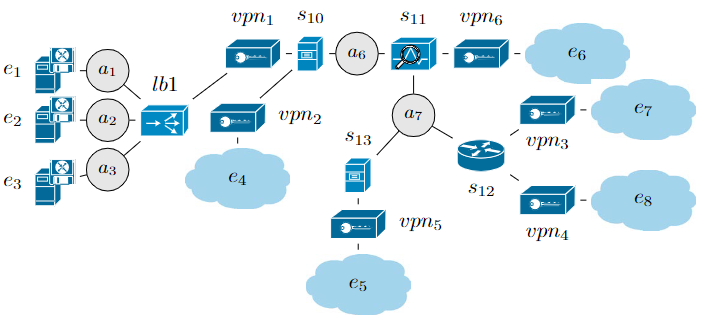
\includegraphics[width=1\textwidth]{VPN_deploy.PNG} 
    \caption{Verefoo Output}
    \label{fig:VPNDeploy}
\end{figure}

As could be imagined, several VPN Gateways were allocated in place of the various Allocation Places defined in the input provided to Verefoo. Given this should be the solution to the problem defined earlier, we will try to test inside the virtual environment the functionality of the various VPN tunnels to make sure that the framework works properly.
Before proceeding, however, it is also important to analyze the various elements that Verefoo has produced. In fact, the framework not only allocates the gateways in the correct places, but also provides an automatic configuration to use. In this specific case, the configuration is as follows:
\\

\begin{table}[ht]
    \centering
    \begin{tabular}{ccccccc}
        \hline
         \# & Action & IPSrc & IPDst & pSrc & pDst & tProto \\
        \hline
        1 & EXIT & 192.168.1.1 & 130.10.0.1 & * & * & ANY \\
        2 & EXIT & 88.80.84.1 & 130.10.0.3 & * & 80 & ANY \\
        3 & EXIT & 40.40.41.1 & 130.10.0.1 & * & 22 & ANY \\
        4 & EXIT & 88.80.84.1 & 130.10.0.1 & * & 80 & ANY \\
        5 & EXIT & 88.80.84.1 & 130.10.0.2 & * & 80 & ANY \\
        6 & ACCESS & 130.10.0.1 & 192.168.1.1 & * & * & ANY \\
        7 & ACCESS & 130.10.0.3 & 88.80.84.1 & 80 & * & ANY \\
        8 & ACCESS & 130.10.0.1 & 40.40.41.1 & 22 & * & ANY \\
        9 & ACCESS & 130.10.0.1 & 88.80.84.1 & 80 & * & ANY \\
        10 & ACCESS & 130.10.0.2 & 88.80.84.1 & 80 & * & ANY\\
        \hline
    \end{tabular}
    \caption{VPN Gateway 1}
    \label{tab:VPN Gateway 1}
\end{table}

\begin{table}[ht]
    \centering
    \begin{tabular}{ccccccc}
        \hline
         \# & Action & IPSrc & IPDst & pSrc & pDst & tProto \\
        \hline
        1 & ACCESS & 40.40.41.1 & 130.10.0.1 & * & 22 & ANY \\
        2 & EXIT & 130.10.0.1 & 40.40.41.1 & 22 & * & ANY \\
        \hline
    \end{tabular}
    \caption{VPN Gateway 2}
    \label{tab:VPN Gateway 2}
\end{table}

\begin{table}[H]
    \centering
    \begin{tabular}{ccccccc}
        \hline
         \# & Action & IPSrc & IPDst & pSrc & pDst & tProto \\
        \hline
        1 & ACCESS & 192.168.1.1 & 130.10.0.1 & * & * & ANY \\
        2 & EXIT & 130.10.0.1 & 192.168.1.1 & * & * & ANY \\
        \hline
    \end{tabular}
    \caption{VPN Gateway 3}
    \label{tab:VPN Gateway 3}
\end{table}

\begin{table}[H]
    \centering
    \begin{tabular}{ccccccc}
        \hline
         \# & Action & IPSrc & IPDst & pSrc & pDst & tProto \\
        \hline
        1 & ACCESS & 192.168.2.1 & 40.40.42.1 & * & * & ANY \\
        2 & EXIT & 40.40.42.1 & 192.168.2.1 & * & * & ANY \\
        \hline
    \end{tabular}
    \caption{VPN Gateway 4}
    \label{tab:VPN Gateway 4}
\end{table}

\begin{table}[H]
    \centering
    \begin{tabular}{ccccccc}
        \hline
         \# & Action & IPSrc & IPDst & pSrc & pDst & tProto \\
        \hline
        1 & ACCESS & 40.40.42.1 & 192.168.2.1 & * & * & ANY \\
        2 & EXIT & 192.168.2.1 & 40.40.42.1 & * & * & ANY \\
        \hline
    \end{tabular}
    \caption{VPN Gateway 5}
    \label{tab:VPN Gateway 5}
\end{table}

\begin{table}[H]
    \centering
    \begin{tabular}{ccccccc}
        \hline
         \# & Action & IPSrc & IPDst & pSrc & pDst & tProto \\
        \hline
        1 & ACCESS & 88.80.84.1 & 130.10.0.1 & * & 80 & ANY \\
        2 & ACCESS & 88.80.84.1 & 130.10.0.2 & * & 80 & ANY \\
        3 & ACCESS & 88.80.84.1 & 130.10.0.3 & * & 80 & ANY \\
        4 & EXIT & 130.10.0.1 & 88.80.84.1 & 80 & * & ANY \\
        5 & EXIT & 130.10.0.2 & 88.80.84.1 & 80 & * & ANY \\
        6 & EXIT & 130.10.0.3 & 88.80.84.1 & 80 & * & ANY \\
        \hline
    \end{tabular}
    \caption{VPN Gateway 6}
    \label{tab:VPN Gateway 6}
\end{table}
